\usection{Lecture 12: Static Games with Incomplete Information}
\newsection
\subsection*{Logistics}
\begin{enumerate}
    \item Exam is on Feb 25. Can bring two double sided handwritten notes. 
    \item Hw 3 posted (shorter than usual homework), practice on dynamic games, due next monday so you can read the solutions.
\end{enumerate}


\subsection*{Recap}
\begin{enumerate}
    \item Dyanmic games with complete information.
\end{enumerate}

Static games with incomplete information are also known as Bayesian Games.
\begin{aexample}{}{}
    There are two firms. Firm 1 is the incumbent and firm 2 is the entrant.
    \begin{itemize}
        \item Firm 1 can decide to build a new factory or not.
        \item Firm 2 can decide to enter or not.
    \end{itemize}
    The cost of building is either 3 or 0. Firm 1 knows the cost but not firm 2. There are two possible scenarios for firm 2.
    \begin{center}
        \begin{tabular}{|c|c c|}
            \hline High cost & enter & not enter \\
            \hline 
            build & (0,-1) & (2,0)\\
            \hline
            not build & \textcolor{red}{(2,1)} & (3,0)\\\hline
        \end{tabular} 
        \linebreak[3pt]
        
        \begin{tabular}{|c|c c|}
            \hline Low cost & enter & not enter \\
            \hline 
            build & (3,-1) & \textcolor{red}{(5,0)}\\
            \hline
            not build & (2,1) & (3,0)\\\hline
        \end{tabular}
    \end{center}
\end{aexample}
The incumbent always knows whether to build or not build, as there is a dominant strategy. The entrant needs to estimate the probability of high cost as $p$.
The payoff of entering is $p-(1-p)=2p-1$. The payoff of not entering is $0$. So the threshold probability is $1/2$. Enter if above $1/2$, don't enter if below.

Now suppose we edit the game so that the payoffs are now 
\begin{center}
    \begin{tabular}{|c|c c|}
        \hline High cost & enter & not enter \\
        \hline 
        build & (0,-1) & (2,0)\\
        \hline
        not build & \textcolor{red}{(2,1)} & (3,0)\\\hline
    \end{tabular} 
    \linebreak[3pt]
    
    \begin{tabular}{|c|c c|}
        \hline Low cost & enter & not enter \\
        \hline 
        build & (1.5,-1) & \textcolor{black}{(3.5,0)}\\
        \hline
        not build & (2,1) & (3,0)\\\hline
    \end{tabular}
\end{center}

Now the incumbent does not have a dominant strategy in the low cost situation, so the incumbent needs to have a belief on the entrant's belief...? and the entrant needs to have a belief on the incumbent's belief on the entrant's belief... 

\subsection*{Harsanyi}

Idea: There is an intiial move in game by `nature' that determines the player's types. Moreover, everyone knows the common prior used by Nature. 
\begin{center}
    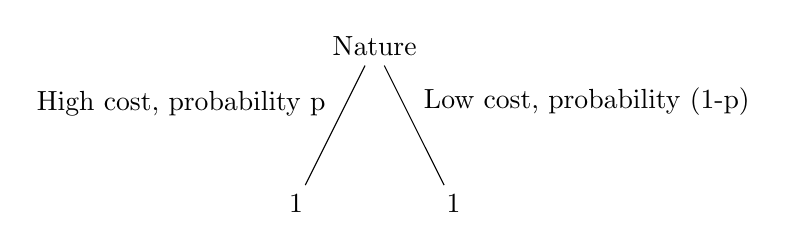
\begin{tikzpicture}
        \node (A) at (0,0){Nature};
        \node(B) at (-1,-2) {1};
        \node(C) at (1,-2) {1};
        \draw (A) edge  node[midway, above left]{High cost, probability p}(B);
        \draw (A) edge  node[midway, above right]{Low cost, probability (1-p)}(C);
    \end{tikzpicture}\end{center}

Let $x$ be the probability of building if the cost is low. Let $y$ be player 2's probability of entering.
Player 2's expected payoff for entering is \[
p +(1-p)(x)(-1)+ (1-p)(1-x) = (1-p)(1-2x)+p.
\]
Not entering payoff is $0$.
SO player 2 should set $y=1$ if $x\leq 1/2(1-p)$.
Similarly for player 1, want $x=1$ if $y<0.5$ and $x=0$ if $y>0.5$.

So if $1/2(1-p)\leq 1\iff p<1/2$ we have two extra equilibirum (one mixed, one (build, don't enter)).


\definition{Bayesian Game}{
    A \textbf{Bayesian game} (Normal form) consists of \begin{itemize}
        \item A set of players $R$.
        \item A set of actions $S_r$ for each $r\in R$.
        \item A set of types for each player $\theta_r\in \Theta_r$. 
        \item A payoff function $\pi_r(s_1,\ldots,s_R, \theta_1,\ldots, \theta_R)$.
        \item A joint distribution $p(\theta_1,\ldots,\theta_R)$.
        \item Optional: A signal to each player that randomly depends on types.
    \end{itemize}
    You might not know about your type. The `signal' gives some information about the type.
}
\begin{remark}
    The joint distirbution is known to all players. 
\end{remark}
\begin{aexample}{}{}
    Nature can choose high or low cost with probability $p_1$ and $(1-p_1)$. Player 1 does not know it, but instead gets a signal with $(1-\epsilon)$ accuracy.
    Probability of being high given a high signal is \[
    \frac{p_1(1-\epsilon)}{\epsilon (1-p_1) + (1-\epsilon)p_1}.
    \]
\end{aexample}

\definition[]{}{
    A pure strategy in a Bayesian game where players can see their own type is a map \[
    \sigma_r:\Theta_r\to S_r
    \]
    i.e. an action for every type.

    A Bayes-Nash equilibrium (BNE) is \[
    \sigma_r(\theta_r)\in\arg \max_{s'_r\in S_r} \sum_{\theta_{-r}} p(\theta_{-r}|\theta_r)\pi_r(s_r,s_{-r},\theta_r,\theta_{-r}). 
    \]
    That is no one can unilaterally improve their payoff by changing the response (to a type).
}
\theorem[]{}{
    A bayesian game with finite strategy set and types has a mixed strategy Nash equilibrium.
}
\begin{proof}
    Expand the strategy set to be functions \[
    \sigma_r:\Theta_r\to S_r.
    \]
    This is finite. Thus this is a finite game and has a nash equilibrium.
\end{proof}
 

\begin{aexample}{Harsanyi mixed strategy justification}{}
    \begin{center}
        \begin{tabular}{|c|c c|}
            \hline  & A & B  \\
            \hline 
            A & (2,1) & (0,0)\\
            \hline
             B & (0,0) & (1,2)\\\hline
        \end{tabular} 
    \end{center}
    We have a mixed Nash equilibrium (2/3,1/3), (1/3,2/3).
    Now we preturb the payoffs by a bit.
    \begin{center}
        \begin{tabular}{|c|c c|}
            \hline  & A & B  \\
            \hline 
            A & (2+$t_A$,1) & (0,0)\\
            \hline
             B & (0,0) & (1,2+$t_B$)\\\hline
        \end{tabular} 
    \end{center}
    where $t_A,t_B$ are iid, chosen uniformly on the interval $[0,x]$. $t_A$ and $t_B$ are known by each player respectivey.
    Notice player 1's payoff for playing $A$ is monotonically increasing in $t_A$. Thus we would expect that player 1 plays $A$ if $t_A>c_A$. Similarly, player 2 plays $B$ if $t_B>c_B$.
    
    So player 1's payoff for choosing A is \[
    (2+t_A)c_B/x
    \]
    Payoff choosing B is\[
    1-c_B/x
    \]
    so is indifferent when \[
        (2+t_A)c_B/x=1-c_B/x\implies t_A = x/c_B-3
    \]
    If $c_A=c_B$, will get \[
    c_A=c_B=\frac{-3+\sqrt{9+4x}}{2}.
    \]
    In this case, player 1 plays $A$ with probability \[
    1-\frac{c_A}{x} = 1-\frac{-3+\sqrt{9+4x}}{2x} \to \frac{2}{3} 
    \]as 
    $x\to 0$. This gives us the mixed strategy equilibria. That is, mixed strategies are just pure strategies in the Bayesian game with very small perturbations.
\end{aexample}